\documentclass{beamer}

\usepackage[utf8]{inputenc}
\usepackage[T1]{fontenc}
\usepackage{listings}

%% Choose a theme from one of the following:
% AnnArbor, Antibes, Bergen, Berkeley, Berlin, Boadilla, boxes, CambridgeUS
% Copenhagen, Darmstadt, default, Dresden, Frankfurt, Goettingen, Hannover
% Ilmenau, JuanLesPins, Luebeck, Madrid, Malmoe, Marburg, Montpellier,
% PaloAlto, Pittsburgh, Rochester, Singapore, Szeged, Warsaw
%\usetheme{Warsaw}

\setbeamercovered{transparent}

\hypersetup{pdfpagelabels=true}

\lstset{ 
language=Python,
breaklines=true,   
basicstyle=\ttfamily,
keywordstyle=\color{keywordcolor},
        commentstyle={\color{commentcolor}\itshape},
        stringstyle={\color{stringcolor}\underbar},
        identifierstyle=\color{idcolor},numbers=left,
        xleftmargin=2em,framerule=0.8pt,
        stepnumber=1,frame=tlrb,showstringspaces=false,
        firstnumber=1,numberstyle=\ttfamily,backgroundcolor=\color{bg}}


%% Choose one of the following color themes or go with the default
% albatross, beaver, beetle, crane, default, dolphin, dove, fly
% lily, orchid, rose, seagull, seahorse sidebartab, structure
% whale, wolverine
\usecolortheme{dove}

\title[Sound Evolution] {Using genetic algorithms to evolve \emph{aesthetic} sounds.}
\subtitle{Humans as a fitness function}

\titlegraphic{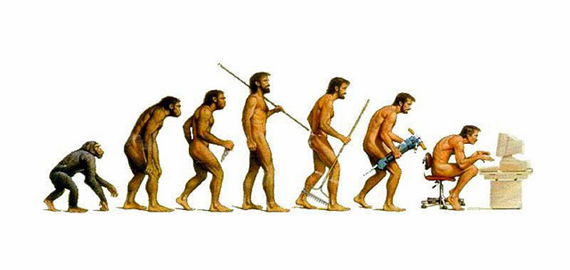
\includegraphics[height=3cm]{images/evolution}}

\author[Duncan, Matthias, Rafael, Mirko \& Stephan] { \\\texttt{..@bccn-berlin.de}} 
\date[SS 2010] {\today}

\pgfdeclareimage[height=0.8cm]{university-logo}{images/bccn_logo.png}
\logo{\pgfuseimage{university-logo}}

\beamerdefaultoverlayspecification{<1->}



\begin{document}

\frame{\titlepage}

\begin{frame}
	\frametitle{Duncan lutscht Schwaenze}
	\framesubtitle{in der Hoelle}
	
\end{frame}


\section{Background} % (fold)
\label{sg:sec:background}

\begin{frame}
	\frametitle{Genetic algorithms}
	\framesubtitle{the idea}
	
	\begin{itemize}
		\item<1-> use the principles of evolution (crossover, mutation, selection)
		to solve optimization problems
		\item<2-> this methods are successfully used in (engineering, robotics, network routing,
		automated joke generation) 
		\item<3-> main problem often to find and design a fitness function
	\end{itemize}
\end{frame}

\begin{frame}
	\frametitle{inspiration}
	\framesubtitle{GE in art}
	
	\begin{itemize}
		\item<1-> synthesizer parameter fitting
		\item<2-> image approximation (compression)
		\item<3-> picbreeder
	\end{itemize}
\end{frame}

\begin{frame}
	\frametitle{inspiration}
	\framesubtitle{synthesizer parameter fitting}

	even if you know that a certain model is capable of performing a sound
	it might be hard to find the right parameters.
	
	parameters could be found
\end{frame}


% section background (end)


\section{The idea} % (fold)
\label{sg:sec:the_idea}

\begin{frame}
	\frametitle{The idea}
	\framesubtitle{a human fitness function}
	
\end{frame}

% section the_idea (end)


\section{The genome} % (fold)
\label{sg:sec:the_genome}

% section the_genome (end)


\section{Implementation} % (fold)
\label{sg:sec:imple}

% section imple (end)

% NOTE here demonstration


\section{Outlook, many more ideas} % (fold)
\label{sg:sec:outlook_many_more_ideas}

% section outlook_many_more_ideas (end)

% TODO add a proper bibliography
%http://en.wikipedia.org/wiki/Computational_humor



\end{document}
